\documentclass{article}
\usepackage[utf8]{inputenc}
\usepackage{indentfirst}
\usepackage{graphicx}
\usepackage{multirow}
\usepackage{hyperref}
\usepackage{mathtools}
\usepackage{caption}
%\usepackage{amssymb,amsmath}
\usepackage{setspace}
\usepackage{geometry}
\usepackage{graphicx}
\usepackage{siunitx}
\usepackage{amsmath}
\usepackage{amssymb}
\usepackage{enumerate}
\usepackage{multirow}
\usepackage{indentfirst}
\usepackage{float}
\usepackage{float}
\usepackage{listings}
\usepackage{enumitem}
\usepackage{listings}
\usepackage{color}
\usepackage{xcolor}

\usepackage{tabularx}

\usepackage{amsmath}
\graphicspath{ {images/} }
\thispagestyle{empty}
\begin{document}
\begin{titlepage}

\begin{center}


\includegraphics[height=1.0in]{logo}

{
\vspace{0.8cm}
\Large
\textsc{VE281 Data Structure} \\[0.5cm]
}



{
\Huge
\textsc{REPORT OF\\ PROGRAM PROJECT 1} \\[0.2cm]
}

{
\vspace{0.01cm}
\middle
\textsc{Sorting}\\[0.8cm]
}

{
\large

\textsc{Group 8}\\[2.6cm]
\textsc{Name and ID}\\[0.3cm]

\begin{tabular}{cc}

Sijun \textsc{Zhang} & 516370910155 \\ [4cm]%这里加了名字以后要调整一下[4cm]这个参数;



Professor: & Weikang Qian \\
\end{tabular}
}

\vspace{1.0cm}

{\large \today}\\

\end{center}

\end{titlepage}

\section{introduction}
In this report, we will discuss the time complexity of different sorting algorithms, which includes Bubble Sort, Inserting Sort, Selection Sort, Merge Sort and Quick Sorts. We test their time efficiency by input 50-, 500-, 5000-, 50000-, 500000- and 1000000-size of integers array, which is generated by mrand48() and repeat each size for five times. Then we could get Time-Size dependency graph to confirming our theoretical time complexities.

By the way, we also test special cases: the sorted array, the reversed array and the uniform array, which somehow show the extreme value of time consuming. 

All the input cases are generated by generate.cpp, which is attached in the appendix.

\section{Normal Array Performance Analysis}
% Table generated by Excel2LaTeX from sheet 'Sheet1'
\begin{table}[htbp]
  \centering
    \begin{tabular}{lrrrrrr}
    \multicolumn{7}{c}{Bubble Sort} \\
    Size  & 50    & 500   & 5000  & 50000  & 500000  & 100000  \\\hline
    1st   & 0.000003  & 0.000005  & 0.000224  & 0.032255  & 3.385270  & 12.906000  \\
    2nd   & 0.000003  & 0.000005  & 0.000203  & 0.030671  & 3.284240  & 12.824300  \\
    3rd   & 0.000001  & 0.000014  & 0.000249  & 0.032633  & 3.253110  & 12.835300  \\
    4th   & 0.000002  & 0.000006  & 0.000470  & 0.031794  & 3.256230  & 12.800500  \\
    5th   & 0.000001  & 0.000006  & 0.000272  & 0.027053  & 3.253480  & 12.837100  \\
    Average & 0.000002  & 0.000007  & 0.000284  & 0.030881  & 3.286466  & 12.840640  \\
    \end{tabular}%
  \label{tab:addlabel}%
\end{table}%

% Table generated by Excel2LaTeX from sheet 'Sheet1'
\begin{table}[htbp]
  \centering
    \begin{tabular}{lrrrrrr}
    \multicolumn{7}{c}{Insertion Sort} \\
    Size  & 50    & 500   & 5000  & 50000  & 500000  & 100000  \\\hline
    1st   & 0.000004  & 0.000007  & 0.000075  & 0.006953  & 0.321603  & 1.514920  \\
    2nd   & 0.000000  & 0.000003  & 0.000075  & 0.004790  & 0.448079  & 1.352470  \\
    3rd   & 0.000001  & 0.000003  & 0.000060  & 0.005318  & 0.394147  & 1.317350  \\
    4th   & 0.000002  & 0.000002  & 0.000040  & 0.003400  & 0.314955  & 1.323330  \\
    5th   & 0.000002  & 0.000003  & 0.000039  & 0.003948  & 0.336799  & 1.307210  \\
    Average & 0.000002  & 0.000004  & 0.000058  & 0.004882  & 0.363117  & 1.363056  \\
    \end{tabular}%
  \label{tab:addlabel}%
\end{table}%

% Table generated by Excel2LaTeX from sheet 'Sheet1'
\begin{table}[htbp]
  \centering
    \begin{tabular}{lrrrrrr}
    \multicolumn{7}{c}{Selection Sort} \\
    Size  & 50    & 500   & 5000  & 50000  & 500000  & 100000  \\ \hline
    1st   & 0.000001  & 0.000006  & 0.000145  & 0.006154  & 0.698495  & 2.401340  \\
    2nd   & 0.000002  & 0.000006  & 0.000221  & 0.005947  & 0.601475  & 2.365530  \\
    3rd   & 0.000002  & 0.000007  & 0.000135  & 0.010497  & 0.768771  & 2.367100  \\
    4th   & 0.000001  & 0.000005  & 0.000135  & 0.010663  & 0.583812  & 2.337060  \\
    5th   & 0.000001  & 0.000007  & 0.000148  & 0.009445  & 0.671227  & 2.373700  \\
    Average & 0.000001  & 0.000006  & 0.000157  & 0.008541  & 0.664756  & 2.368946  \\
    \end{tabular}%
  \label{tab:addlabel}%
\end{table}%


\begin{table}[htbp]
  \centering
    \begin{tabular}{lrrrrrr}
    \multicolumn{7}{c}{Merge Sort} \\
    Size  & 50    & 500   & 5000  & 50000  & 500000  & 100000  \\ \hline
    1st   & 0.000015  & 0.000020  & 0.000190  & 0.001564  & 0.014325  & 0.027561  \\
    2nd   & 0.000014  & 0.000016  & 0.000259  & 0.001042  & 0.012350  & 0.021918  \\
    3rd   & 0.000009  & 0.000027  & 0.000088  & 0.001592  & 0.010875  & 0.019424  \\
    4th   & 0.000014  & 0.000028  & 0.000087  & 0.001624  & 0.011109  & 0.030057  \\
    5th   & 0.000011  & 0.000016  & 0.000167  & 0.001007  & 0.010301  & 0.019932  \\
    Average & 0.000013  & 0.000021  & 0.000158  & 0.001366  & 0.011792  & 0.023778  \\
    \end{tabular}%
  \label{tab:addlabel}%
\end{table}%


\begin{table}[htbp]
  \centering
    \begin{tabular}{lrrrrrr}
    \multicolumn{7}{c}{Quick with Extra Space Sort} \\
    Size  & 50    & 500   & 5000  & 50000  & 500000  & 100000  \\ \hline
    1st   & 0.000012  & 0.000041  & 0.000194  & 0.001390  & 0.010501  & 0.017799  \\
    2nd   & 0.000010  & 0.000012  & 0.000126  & 0.000740  & 0.010957  & 0.030540  \\
    3rd   & 0.000010  & 0.000025  & 0.000139  & 0.000902  & 0.013921  & 0.015684  \\
    4th   & 0.000006  & 0.000088  & 0.000125  & 0.001220  & 0.011950  & 0.026427  \\
    5th   & 0.000006  & 0.000014  & 0.000119  & 0.000821  & 0.010377  & 0.027992  \\
    Average & 0.000009  & 0.000036  & 0.000141  & 0.001015  & 0.011541  & 0.023688  \\
    \end{tabular}%
  \label{tab:addlabel}%
\end{table}%


\begin{table}[htbp]
  \centering
    \begin{tabular}{lrrrrrr}
    \multicolumn{7}{c}{Quick In Place Sort} \\
    Size  & 50    & 500   & 5000  & 50000  & 500000  & 100000  \\ \hline
    1st   & 0.000012  & 0.000017  & 0.000038  & 0.000428  & 0.004147  & 0.010627  \\
    2nd   & 0.000009  & 0.000008  & 0.000039  & 0.000364  & 0.004633  & 0.009025  \\
    3rd   & 0.000009  & 0.000014  & 0.000039  & 0.000362  & 0.004321  & 0.011141  \\
    4th   & 0.000006  & 0.000021  & 0.000043  & 0.000445  & 0.005321  & 0.010552  \\
    5th   & 0.000006  & 0.000015  & 0.000042  & 0.000360  & 0.005406  & 0.011200  \\
    Average & 0.000008  & 0.000015  & 0.000040  & 0.000392  & 0.004766  & 0.010509  \\
    \end{tabular}%
  \label{tab:addlabel}%
\end{table}%


\begin{table}[htbp]
  \centering
    \begin{tabular}{l|rrrrrr}
    \multicolumn{7}{c}{The comparison result.} \\
          & 50    & 500   & 5000  & 50000  & 500000  & 100000  \\ \hline
    Bubble & 0.000002 & 0.0000072 & 0.0002836 & 0.0308812 & 3.286466 & 12.84064 \\
    Insertion & 0.0000018 & 0.0000036 & 0.0000578 & 0.0048818 & 0.3631166 & 1.363056 \\
    Selection & 0.0000014 & 0.0000062 & 0.0001568 & 0.0085412 & 0.664756 & 2.368946 \\
    Merge & 0.0000126 & 0.0000214 & 0.0001582 & 0.0013658 & 0.011792 & 0.0237784 \\
    Quick\_Extra & 0.0000088 & 0.000036 & 0.0001406 & 0.0010146 & 0.0115412 & 0.0236884 \\
    Quick\_In\_Place & 0.0000084 & 0.000015 & 0.0000402 & 0.0003918 & 0.0047656 & 0.010509 \\
    \end{tabular}%
  \label{tab:addlabel}%
\end{table}%

\begin{center}
    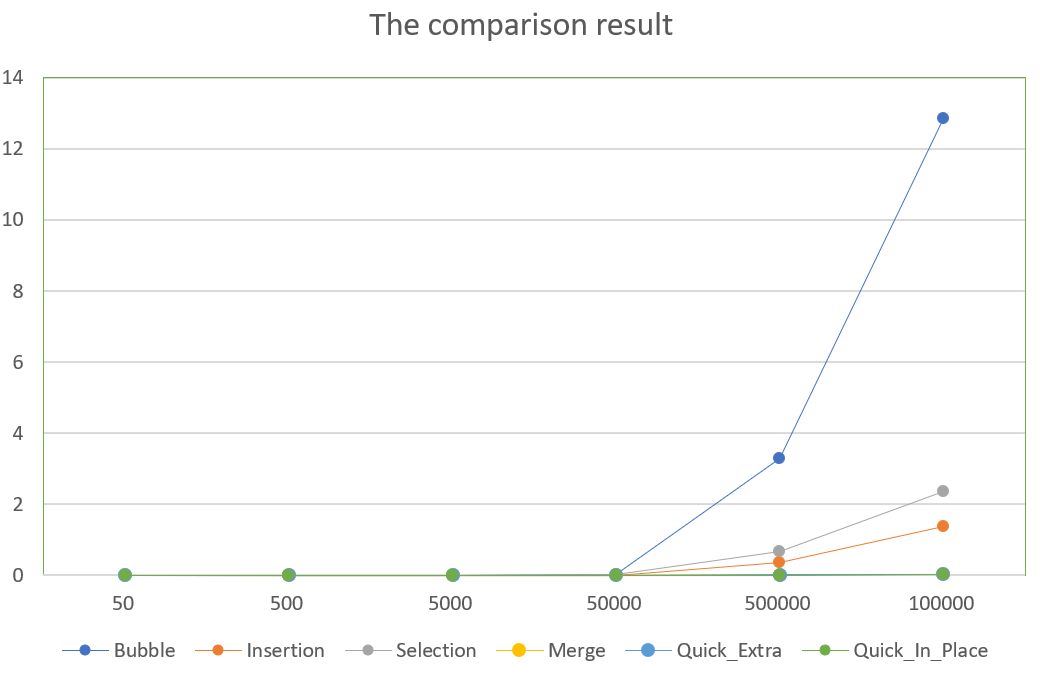
\includegraphics[height = 9cm]{result1.PNG}
    \caption{The result in normal size}
\end{center}

We find it is hard to distinguish the difference among the sorting algorithms of $O(nlogn)$, so we could transform the perpendicular coordinate to log size, then we could find the exact difference in log size

% Table generated by Excel2LaTeX from sheet 'Sheet1'
\begin{table}[htbp]
  \centering
    \begin{tabular}{l|rrrrrr}
    \multicolumn{7}{c}{The comparison result in Log Size} \\
          & 50    & 500   & 5000  & 50000  & 500000  & 100000  \\ \hline
    Bubble & -5.69897 & -5.14267 & -3.54729 & -1.51031 & 0.516729 & 1.108587 \\
    Insertion & -5.74473 & -5.4437 & -4.23807 & -2.31142 & -0.43995 & 0.134514 \\
    Selection & -5.85387 & -5.20761 & -3.80465 & -2.06848 & -0.17734 & 0.374555 \\
    Merge & -4.89963 & -4.66959 & -3.80079 & -2.86461 & -1.92841 & -1.62382 \\
    Quick\_Extra & -5.05552 & -4.4437 & -3.85201 & -2.99371 & -1.93775 & -1.62546 \\
    Quick\_In\_Place & -5.07572 & -4.82391 & -4.39577 & -3.40694 & -2.32188 & -1.97844 \\
    \end{tabular}%
  \label{tab:addlabel}%
\end{table}%

\begin{center}
    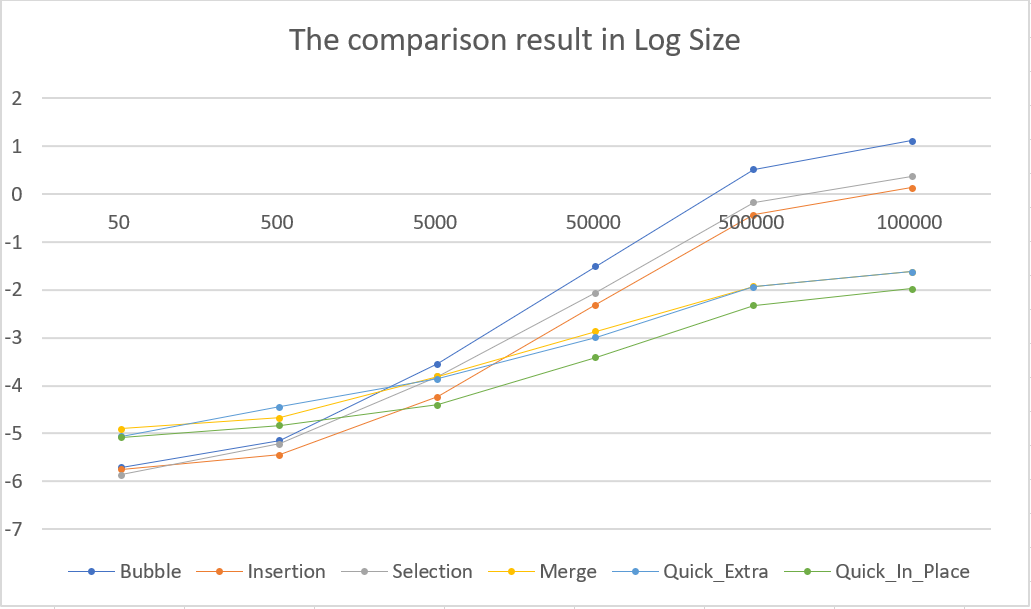
\includegraphics[height = 9cm]{result2.PNG}
    \caption{The result in Log size}
\end{center}

\subsection{Discussion}

Thus we could withdraw the following conclusion

\begin{itemize}
    \item In relative short array (size less than 500), Bubble, Insertion and Selection Sorts perform better than Merge and Quick sorts
    \item In large scale (greater than 5000) Merge and Quick sorts have better performances.
    \item In large scale, the Bubble sort has the worst performance and the Quick Sort In Place perform best.
    \item Quick Sort In Place perform better than the version need extra space.
\end{itemize}

\section{Special Cases Test}
Although we have got the result of normal unsorted array and come to conclusion that Quick Sort In Place has the best performance in large input size, it doesn't mean that other sort is useless. In the extreme cases, the performance of different sort is also different to the normal cases. 

In the previous part, we find the normal digits size is hard to compare, so we use log size in the following graph.

\subsection{Input Sorted Array}
In this part, we input an already sorted array (from 0 to size - 1), to test the case that if the input array is almost sorted, how the sorting algorithms will perform.

% Table generated by Excel2LaTeX from sheet 'Sheet1'
\begin{table}[H]
  \centering
    \begin{tabular}{l|rrrrrr}
    \multicolumn{7}{c}{The comparison result in Log Size of Sorted Array} \\
          & 50    & 500   & 5000  & 50000  & 500000  & 100000  \\ \hline
    Bubble & -6    & -5.65758 & -4.01502 & -2.17057 & -0.19416 & 0.401768 \\
    Insertion & -5.79588 & -5.74473 & -5.52288 & -5.0655 & -4.19382 & -3.93405 \\
    Selection & -5.74473 & -5.55284 & -4.01412 & -2.1429 & -0.21538 & 0.374323 \\
    Merge & -5    & -4.69037 & -3.87095 & -3.03858 & -2.04168 & -1.76054 \\
    Quick\_Extra & -5.00877 & -4.77469 & -3.87877 & -2.97675 & -2.0054 & -1.69087 \\
    Quick\_In\_Place & -5.20761 & -5.08619 & -4.48678 & -3.67695 & -2.70695 & -2.38084 \\
    \end{tabular}%
  \label{tab:addlabel}%
\end{table}%

\begin{center}
    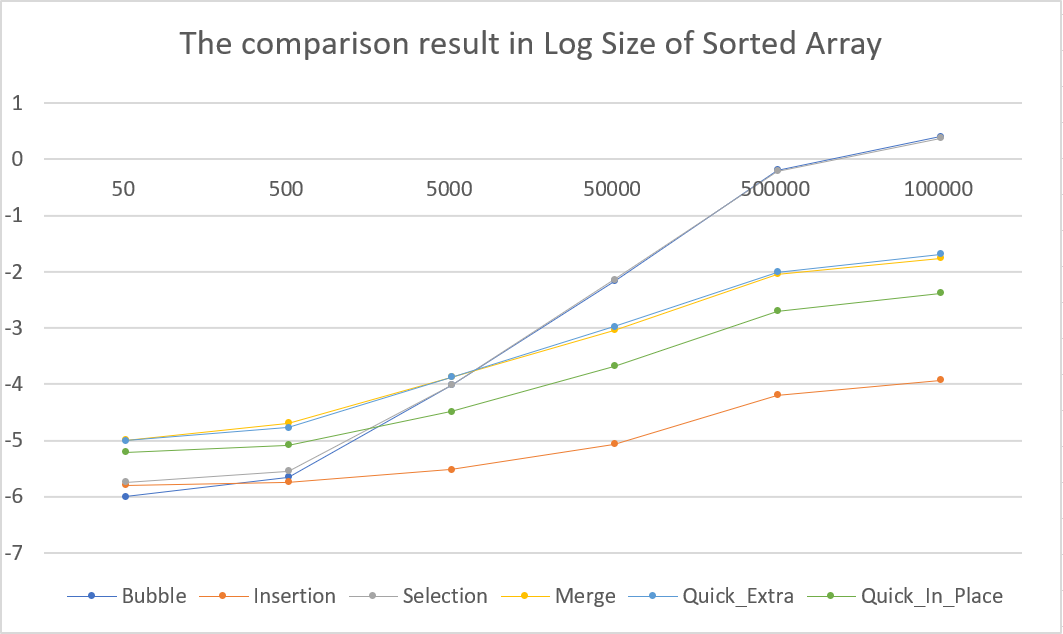
\includegraphics[height = 9cm]{result3.PNG}
    \caption{The result in Log size of Sorted Array}
\end{center}


\subsection{Input Reversed Array}
In this part, we input a reversed array (with size - 1 to zero).

% Table generated by Excel2LaTeX from sheet 'Sheet1'
\begin{table}[H]
  \centering
    \begin{tabular}{l| rrrrrr}
    \multicolumn{7}{c}{The comparison result in Log Size of Reversed Array} \\
          & 50    & 500   & 5000  & 50000  & 500000  & 100000  \\ \hline
    Bubble & -5.79588 & -5.61979 & -3.91364 & -2.03077 & -0.0133 & 0.577783 \\
    Insertion & -5.92082 & -5.74473 & -4.07572 & -2.19485 & -0.13658 & 0.415019 \\
    Selection & -5.74473 & -5.4437 & -4.06449 & -2.15171 & -0.1996 & 0.3919 \\
    Merge & -4.97469 & -4.7167 & -3.95703 & -2.97584 & -2.04055 & -1.71677 \\
    Quick\_Extra & -5.07572 & -4.76955 & -3.99827 & -2.96489 & -2.05503 & -1.64154 \\
    Quick\_In\_Place & -5.23657 & -5.01773 & -4.51999 & -3.69897 & -2.70377 & -2.34781 \\
    \end{tabular}%
  \label{tab:addlabel}%
\end{table}%

\begin{center}
    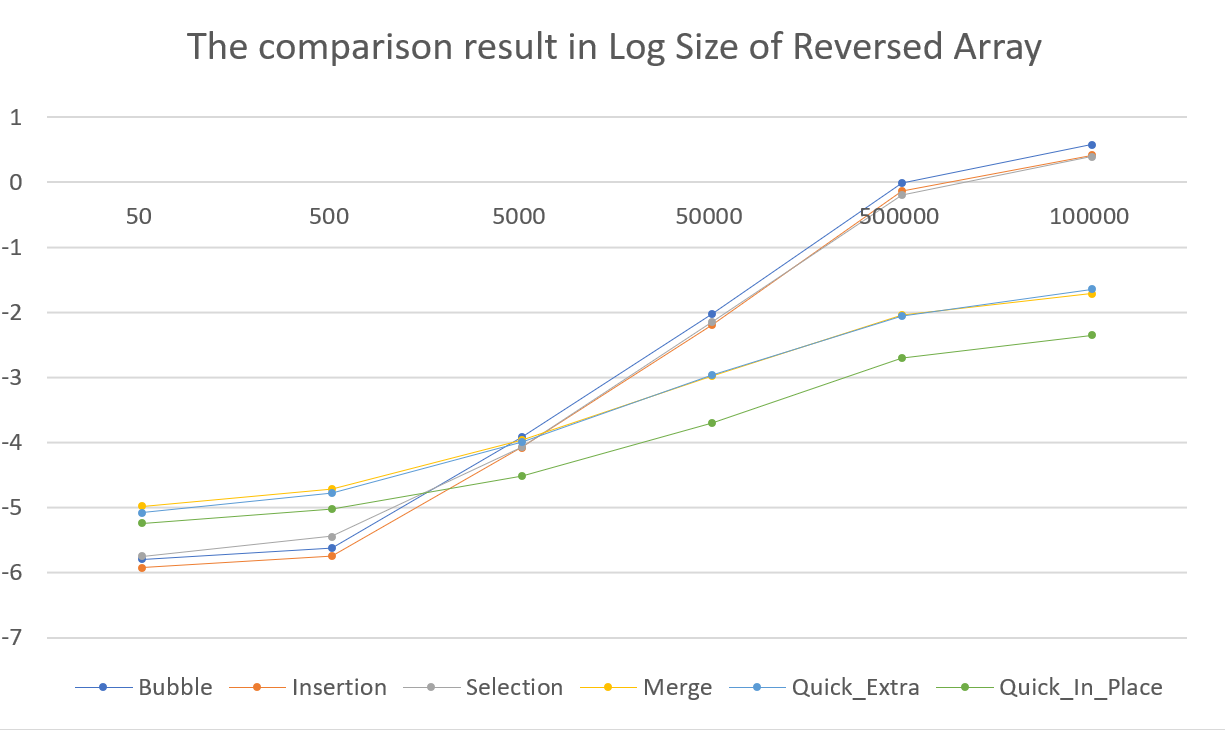
\includegraphics[height = 9cm]{result4.PNG}
    \caption{The result in Log size of Reversed Array}
\end{center}

\subsection{Input Uniform Array with all zeros}
In this part, we input an array with all zeros, to test the cases that if we input an array that most elements are same.

% Table generated by Excel2LaTeX from sheet 'Sheet1'
\begin{table}[H]
  \centering
    \begin{tabular}{l | rrrrrr}
    \multicolumn{7}{c}{The comparison result in Log Size of Uniform Array} \\
          & 50    & 500   & 5000  & 50000  & 500000  & 100000  \\ \hline
    Bubble & -6    & -5.61979 & -4.058489 & -2.1928846 & -0.194957874 & 0.405635566 \\
    Insertion & -5.92082 & -5.74473 & -5.420216 & -4.9665762 & -4.229147988 & -3.938547521 \\
    Selection & -5.79588 & -5.49485 & -4.056505 & -2.2368566 & -0.197363903 & 0.373090469 \\
    Merge & -4.76955 & -4.75449 & -3.931814 & -2.9664154 & -1.948693089 & -1.696661362 \\
    Quick\_Extra & -4.9914 & -4.66959 & -3.329754 & -1.4590802 & 0.521699426 & 1.044689072 \\
    Quick\_In\_Place & -5.19382 & -5.13077 & -3.876802 & -2.0564461 & -0.166810035 & 0.42335042 \\
    \end{tabular}%
  \label{tab:addlabel}%
\end{table}%


\begin{center}
    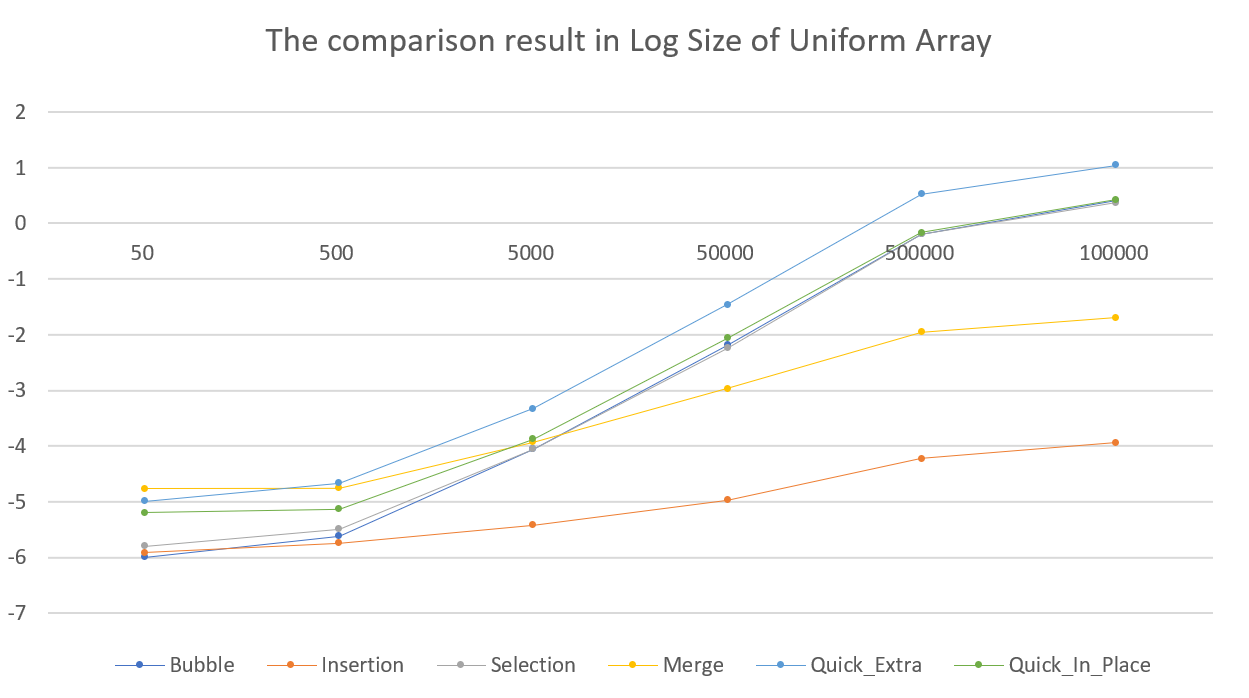
\includegraphics[height = 9cm]{result5.PNG}
    \caption{The result in Log size of Reversed Array}
\end{center}

\subsection{Discussion}

We find in Uniform input and Sorted input, Insertion Sort has the best performance whether in large scale or small scale. Moreover the Merge sort has the most stable performance whenever the input changes. 

\section{Conclusion}

We have obtained the characteristics and performance of the six sorting algorithms. Merge Sort has the most steady performance, and Quick Sorts' vary a lot. In some special cases, Insertion Sort is also a good choice due to small probability to swap. Overall, in normal cases, Quick Sort In Place is the best choice. 



\section{Appendix}


\subsection{generate.cpp}
\begin{lstlisting}[title=generate.cpp, frame=shadowbox]

#include <iostream>
#include <fstream>
#include <sstream>
#include <string>
#include <cstdlib>
#include <climits>
#include <ctime>
#include <math.h>

using namespace std;

int main(int argc, char*argv[])
{
    srand(unsigned(time(NULL)));
    ofstream oFile;
    int len = pow(10,atoi(argv[3]))/2;
    if (atoi(argv[3]) == 6) len = 100000;
    int tp = atoi(argv[4]);
    if (argc == 5 && tp == 0)
    {
        string file_name(argv[1]);
        oFile.open(file_name);
        oFile << argv[2] << endl;
        oFile << len << endl;
        for (int i = 0; i < len; i++)
        {
            oFile << i << endl;
        }
    }
    else if (argc == 5 && tp == 1)
    {
        string file_name(argv[1]);
        oFile.open(file_name);
        oFile << argv[2] << endl;
        oFile << len << endl;
        for (int i = len - 1 ; i >= 0; i--)
        {
            oFile << i << endl;
        }
    }
    else if (argc == 5 && tp == 2)
    {
        string file_name(argv[1]);
        oFile.open(file_name);
        oFile << argv[2] << endl;
        oFile << len << endl;
        for (int i = len - 1 ; i >= 0; i--)
        {
            oFile << 0 << endl;
        }
    }
    else 
    {
        string file_name(argv[1]);
        oFile.open(file_name);
        oFile << argv[2] << endl;
        oFile << len << endl;
        for (int i = 0; i < len; i++)
        {
            oFile << mrand48() << endl;
        }
    }
    return 0;    
}
\end{lstlisting}



\subsection{main test.cpp}
\begin{lstlisting}[title=main_test, frame=shadowbox]
#include <iostream>
#include <fstream>
#include <sstream>
#include <string>
#include <cstdlib>
#include <climits>
#include <ctime>

using namespace std;


void print(int *arr, int array_length)
{
    for (int i = 0; i < array_length; i++)
    {
         cout << arr[i] << endl;
    }
}

void bubble_sort(int *arr, int array_length)
{
    for (int i = array_length - 2; i >= 0; i--)
    {
        for (int j = 0; j <= i; j++)
        {
            if (arr[j] > arr[j + 1]) swap(arr[j], arr[j+1]);
        }
    }
}

void insertion_sort(int *arr, int array_length)
{
    for (int i = 1; i < array_length; i++)
    {   
        int j = i;
        int temp = arr[j];
        while (1)
        {
            if (j == 0) break;
            if (arr[j - 1] > temp) 
            {
                arr[j] = arr[j-1];
            }
            else break;
            j--;
        }
        arr[j] = temp;
    }
}

void selection_sort(int *arr, int array_length)
{
    for (int i = 0; i < array_length - 1; i++)
    {
        int ipointer = i;
        for (int j = i + 1; j < array_length; j++)
        {
            if (arr[j] < arr[ipointer]) ipointer = j;
        }
        swap(arr[ipointer],arr[i]);
    }
}



void merge(int *arr, int left, int mid, int right)
{
    int * temp = new int[right - left + 1];int j = 0;
    int left_start = left, right_start = mid + 1, i = 0;
    while (left_start <= mid && right_start <= right)
    {
        if (arr[left_start] <= arr[right_start]) 
        {
            temp[i++] = arr[left_start++];
        }
        else 
        {
            temp[i++] = arr[right_start++];
        }
    }
    while (left_start <= mid) temp[i++] = arr[left_start++];
    while (right_start <= right) temp[i++] = arr[right_start++];
    for (j = left; j <= right; j++)
    {
        arr[j] = temp[j - left];
    }

    delete [] temp;
}


void merge_sort(int *arr, int left, int right)
{
    if (left < right)
    {
        int mid = (left + right) / 2;
        merge_sort(arr, left, mid);
        merge_sort(arr, mid + 1, right);
        merge(arr, left, mid, right);
    }
}

int partition_extra(int *arr, const int & left, const int & right)
{
    int pivotat, i;
    int array_length = right - left + 1;
    int *temp = new int[array_length];
    int left_temp = 0, right_temp = right - left;
    //srand(time(0));
    pivotat = rand() % array_length;
    pivotat += left;
    swap(arr[left], arr[pivotat]);
    for (i = left + 1; i <= right; i++)
    {
        if (arr[i] < arr[left]) 
        {
            temp[left_temp++] = arr[i];
        }
        else 
        {
            temp[right_temp--] = arr[i];
        }
    }
    temp[left_temp] = arr[left];
    pivotat = left_temp + left;
    for (i = left; i <= right; i++)
    {
        arr[i] = temp[i - left];
    }
    delete [] temp;
    return pivotat;
}

int partition_in(int *arr, const int & left, const int & right)
{
    int pivotat;
    int array_length = right - left + 1;
    int left_temp = left + 1, right_temp = right;
    //srand(time (0));
    pivotat = rand() % array_length + left;
    swap(arr[left], arr[pivotat]);
    while (left_temp <= right_temp)
    {
        while (arr[left_temp] < arr[left] && left_temp < right) 
        {
            left_temp++;
        }
        while (arr[right_temp] >= arr[left] && right_temp > left) 
        {
            right_temp--;
        }
        if (left_temp >= right_temp) break;
        swap(arr[left_temp], arr[right_temp]);
    }
    swap(arr[left], arr[right_temp]);
    pivotat = right_temp;
    return pivotat;

}

void quick_extra_sort(int *arr, const int & left, const int & right)
{
    if (left < right)
    {
       // cout << "here";
        int pivotat;
        pivotat = partition_extra(arr, left, right);
        quick_extra_sort(arr, left, pivotat-1); 
        quick_extra_sort(arr, pivotat+1, right);
    }
}

void quick_in_sort(int *arr, const int & left, const int & right)
{
    if (left < right)
    {
        int pivotat;
        pivotat = partition_in(arr, left, right);
        quick_in_sort(arr, left,pivotat - 1);
        quick_in_sort(arr,pivotat + 1, right);
    }
}

int main()
{
    ios::sync_with_stdio(false);
    srand(time(NULL));
    int sort_type, array_length;
    double during_time;
    double start, end;
    start = clock();
    cin >> sort_type;
    cin >> array_length;
    int *arr = new int[array_length];
    for(int i = 0; i < array_length; i++)
    {
        cin >> arr[i];
    }
    start = clock();
    if (sort_type == 0)
    {
        bubble_sort(arr, array_length);
    }
    else if (sort_type == 1)
    {
        insertion_sort(arr, array_length);
    }
    else if (sort_type == 2)
    {
        selection_sort(arr, array_length);
    }
    else if (sort_type == 3)
    {
        int left = 0, right = array_length - 1;
        merge_sort(arr, left, right);

    }
    else if (sort_type == 4)
    {
        int left = 0, right = array_length - 1;
        quick_extra_sort(arr, left, right);
    }
    else if (sort_type == 5)
    {
        int left = 0, right = array_length - 1;
        quick_in_sort(arr, left, right);
    }

    end = clock();
    during_time = (end - start) / CLOCKS_PER_SEC;
    //cout << sort_type << endl;
    cout << during_time << endl;
    //print(arr, array_length);
    delete [] arr;
    return 0;
}
\end{lstlisting}
\end{document}
